%\documentclass[fleqn, letterpaper]{amsart}
\documentclass[fleqn, letterpaper]{tufte-handout}
\usepackage{times}
\usepackage{amsmath}
\usepackage{amssymb}
\usepackage{graphicx}
\usepackage{booktabs}
\usepackage{multirow}
\usepackage{listings}
\usepackage{epstopdf}
\usepackage{bm}
%\usepackage[left=1in]{geometry}

\newcommand{\R}{\mathcal{R}}
\newcommand{\E}{\text{E}}
\newcommand{\p}{p_{XY}}
\newcommand{\T}{^\text{T}}
\renewcommand{\arraystretch}{1.5}

\title{Problem Set 4 --- ENCE689E Spring 2014}
\author{David Prentiss}

\begin{document}
\maketitle

\section{Time-varying (Dynamic) Model}

\subsection{(a)}

{\small
\begin{minipage}{\linewidth}
        \lstinputlisting[language=Matlab, caption={Propagation of a linear soil moisture model},
        basicstyle=\ttfamily, label=lst1]{ps5a.m}
\end{minipage}
}

\subsection{(b)}

\begin{figure}
        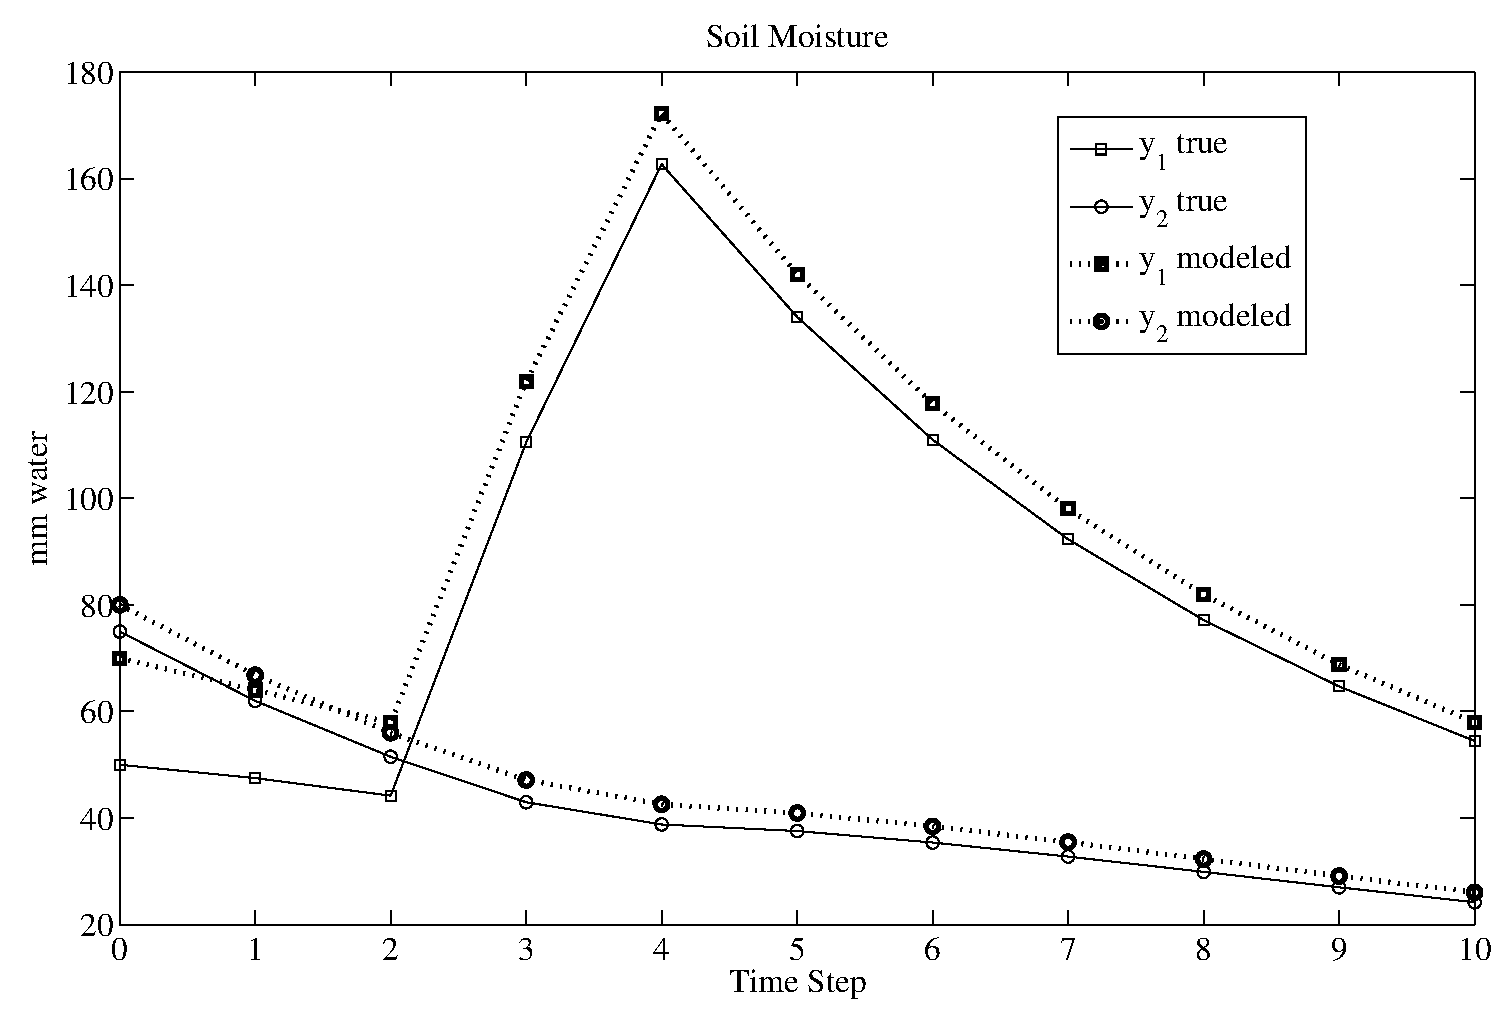
\includegraphics[width=\textwidth]{ps5figb}
        \caption{Plot of $x$}
        \label{exprnd}
\end{figure}

\subsection{(c)}

\[
\bar{\mathbf{y}}_{t+1} = \mathbf{A}\bar{\mathbf{y}}_t + \mathbf{G}\bar{u}_t
\]

\[
\mathbf{C}_{\mathbf{yy}}^{(t+1)} = \mathbf{AC}_{\mathbf{yy}}^{(t)}\mathbf{A}^\intercal + \mathbf{GC}_\mathbf{{uu}}^{(t)}\mathbf{G}^\intercal
\]

\begin{figure}
        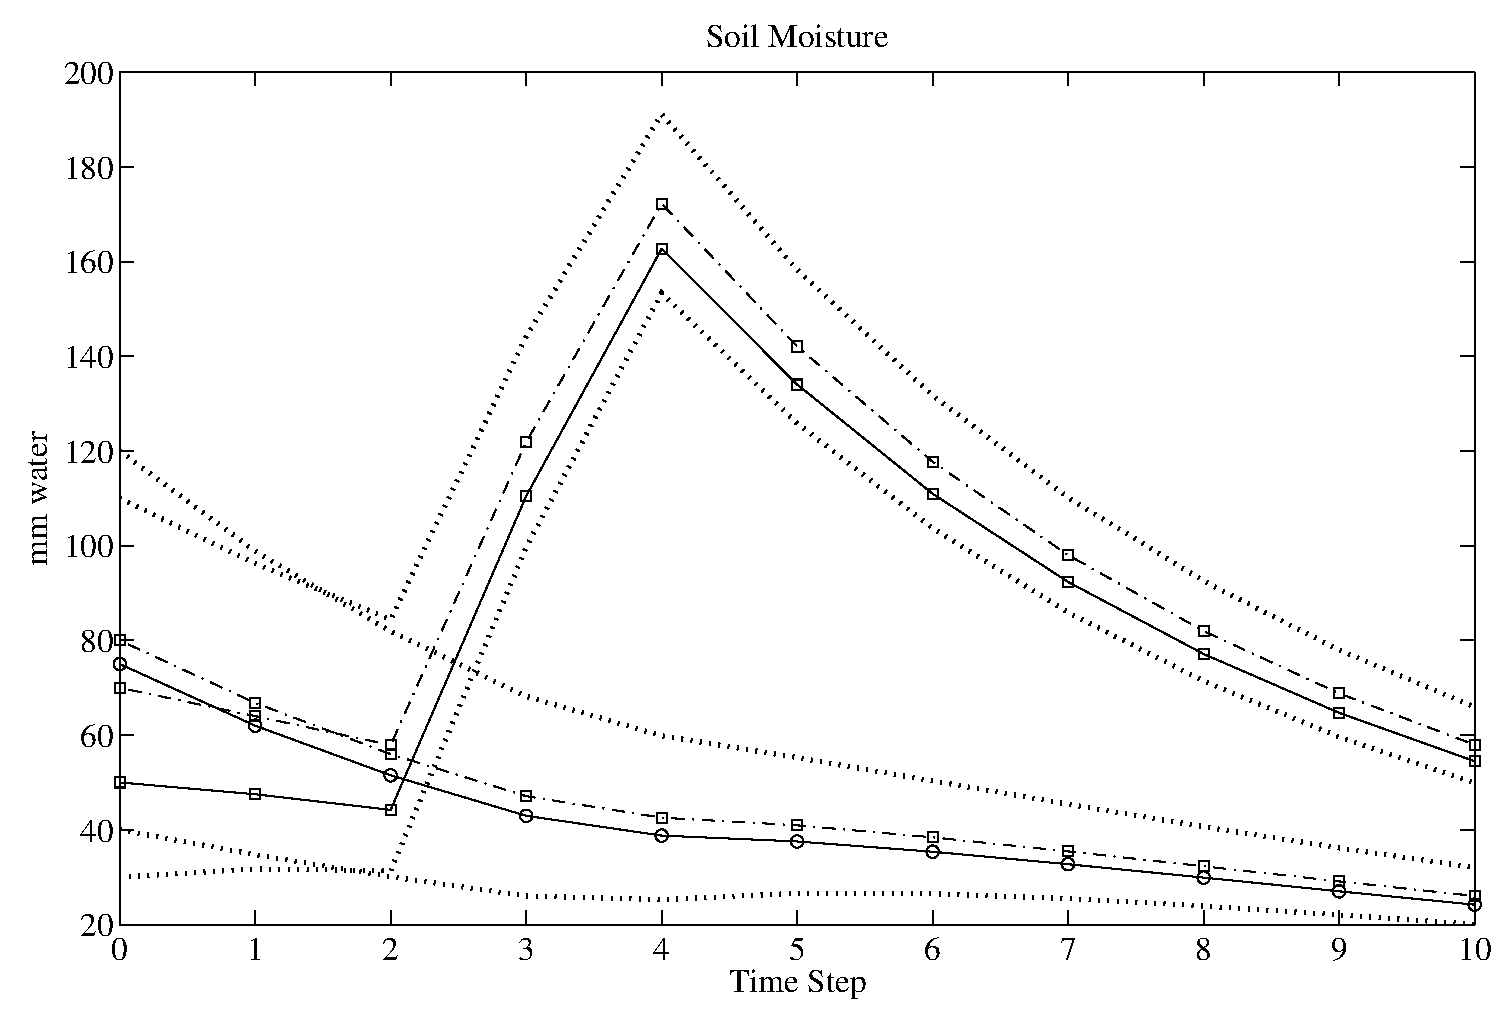
\includegraphics[width=\textwidth]{ps5figc}
        \caption{Plot of $x$}
        \label{exprnd}
\end{figure}

\subsection{(d)}

\subsection{(e)}

Because measurements of moisture are bound below at zero, a Gaussian distribution may not be the best to model the uncertainty of initial conditions. A disribution with a lower bound on its support would be more appropriate. Furthermore, since the probability of moistures close to zero should be decresing in the limit as the moisture approaches zero, a gamma distribution may be more appropriate.

\subsection{(f)}

As with the uncertainty in the initial conditions, the precipitation forcing is bound below at zero. An exponential disribution may be better. 

\subsection{(g)}

Since the model state mean vector $\bar{\mathbf{y}}_t$ is a Gaussian random vector, taking the coefficient matrix $\mathbf{A}$ to contain random variables would mean the transformation $\mathbf{A}\bar{\mathbf{y}}_t$ is no longer linear and the evolving pdf would not, in general be Gaussian.

\end{document}
